\section{Additional Electrical Measurements}

In addition to the current--voltage measurements discussed above, two further electrical tests were performed to probe time-dependent and circuit-level behaviour of the fabricated OFETs. The first test uses a deep-level transient spectroscopy (DLTS)-type experiment to study slow charge relaxation after a gate-bias perturbation~\cite{Lang1974DLTS,Hirwa2015TrapStates}. The second test evaluates whether the device can be biased and operated as a simple voltage amplifier. These measurements are complementary to the transfer and output characteristics: they do not only test the static channel conductance, but also reveal how traps, capacitances, contact effects, and external circuit elements influence the dynamic response of the organic transistor.

\subsection{Deep-level Transient Spectroscopy}



Organic semiconductors usually contain a broad distribution of localized states originating from energetic disorder, impurities, grain boundaries, and interfaces. These states can capture and release charge carriers on time scales that are much longer than the intrinsic carrier transit time~\cite{Hirwa2015TrapStates,Bobbert2012OperationalStability}. As a result, they can contribute to hysteresis, threshold-voltage shifts, slow current relaxation, and bias-stress effects. A DLTS-type transient measurement was therefore used to perturb the device electrically and observe the relaxation of the current after the perturbation.

\begin{figure}[htbp]
\centering
\resizebox{0.55\textwidth}{!}{\begin{circuitikz}[scale=0.5]
\ctikzset{resistor = european}
\ctikzset{tripoles/mos style/arrows}


\draw (-4,-4)--(-4,-5)--(-4,-6) node[rground]{};
\draw (-4,-4)--(-8,-4)--(-8,8)--(8,8)--(8,-4)--(4,-4);
\draw (-4,4)to[short,-*](-8,4);
\draw (4,4)to[short,-*](8,4);

\draw (-10,0)to[crossing,bipoles/crossing/size=0.5](-6,0)--(-4,0);
\draw (4,0)--(6,0)to[crossing,bipoles/crossing/size=0.5](10,0);
\draw (10,0)--(10,10)--(-10,10)--(-10,0);

\draw (0,10)to[short,*-] (0,12) to[R, l={$R_2 = 100\,\mathrm{k\Omega}$}] (0,16);
\draw (0,16) to[R, l={$R_1 = 1\,\mathrm{M\Omega}$}] (0,20);
\draw[red, ->] (0,20) -- (0,22) node[left=1pt]{Input signal};

\draw (0,12)to[short,*-](2,12) to[rmeter,t=V] (2,16)to[short,-*](0,16);

\draw[black, fill = cyan!50, fill opacity = 0.3, line width = 1pt](-5,-5)--(5,-5)--(5,5)--(-5,5)--(-5,-5);

% Gate layer
\filldraw[line width = 1pt,fill = black!40, fill opacity = 0.5]
(-1.5,2.25)--(1.5,2.25) arc[start angle = 180, end angle = -90, radius = 0.75]
--(2.25,0.75)--(4,0.75) arc[start angle = 90, end angle = -90, radius = 0.75]--(2.25,-0.75)
--(2.25,-1.5) arc[start angle = 90, end angle = -180, radius = 0.75] --(-1.5,-2.25)
arc[start angle = 0, end angle = -270, radius = 0.75]--(-2.25,-0.75)
--(-4,-0.75) arc[start angle = -90, end angle = -270, radius = 0.75]--(-2.25,0.75)
--(-2.25,1.5) arc [start angle = -90, end angle = -360, radius = 0.75]
;
\draw[fill = black!40, fill opacity = 0.5, line width = 1pt](-4,-4) circle (0.75);
 \draw[fill = black!40, fill opacity = 0.5, line width = 1pt](-4,4) circle (0.75);
  \draw[fill = black!40, fill opacity = 0.5,line width = 1pt](4,4) circle (0.75);
 \draw[fill = black!40, fill opacity = 0.5,line width = 1pt](4,-4) circle (0.75);

% Insulator
\filldraw[draw=black, fill=blue!80, fill opacity=0.3, line width = 1pt]
(-4.5,-2.7)[sharp corners]--(-4.5,-0.9)[rounded corners=2ex]
--(-2.7,-0.9)--(-2.7,0.9)[sharp corners]--(-4.5,0.9)
--(-4.5,2.7)[rounded corners=2ex]--(-2.7,2.7)[sharp corners]--(-2.7,4.5)
--(2.7,4.5)[rounded corners=2ex]--(2.7,2.7)[sharp corners]--(4.5,2.7)
--(4.5,0.9)[rounded corners=2ex]--(2.7,0.9)--(2.7,-0.9)[sharp corners]--(4.5,-0.9)
--(4.5,-2.7)[rounded corners=2ex]--(2.7,-2.7)[sharp corners]--(2.7,-4.5)
--(-2.7,-4.5)[rounded corners=2ex]--(-2.7,-2.7)[sharp corners]--(-4.5,-2.7)
--cycle;


% Semiconductor layer
\path[fill=green, fill opacity=0.5, draw=green!50!black, line width=1pt]
    (0.7557,2.1193)
    arc[start angle=70.3746, end angle=109.6254, radius=2.25]
    arc[start angle=355.0011, end angle=634.9989, radius=1.5]
    arc[start angle=160.3746, end angle=199.6254, radius=2.25]
    arc[start angle=85.0011, end angle=364.9989, radius=1.5]
    arc[start angle=250.3746, end angle=289.6254, radius=2.25]
    arc[start angle=175.0011, end angle=454.9989, radius=1.5]
    arc[start angle=340.3746, end angle=379.6254, radius=2.25]
    arc[start angle=265.0011, end angle=544.9989, radius=1.5]
    -- cycle;


% Injection pads
\draw[red!90, draw opacity=0.7, line width=1cm, line cap=round, line width = 20pt](-2.25,-2.25) -- (-4,-4);
\draw[red!90, draw opacity=0.7, line width=1cm, line cap=round, line width = 20pt](2.25,-2.25) -- (4,-4);
\draw[red!90, draw opacity=0.7, line width=1cm, line cap=round, line width = 20pt](-2.25,2.25) -- (-4,4);
\draw[red!90, draw opacity=0.7, line width=1cm, line cap=round, line width = 20pt](2.25,2.25) -- (4,4);



% Contact pads
\draw[fill=orange, line width = 1pt](-4,-4) circle (0.75) node []{4};
 \draw[fill=orange, line width = 1pt](-4,4) circle (0.75) node []{3};
  \draw[fill=orange,line width = 1pt](4,4) circle (0.75) node []{2};
 \draw[fill=orange,line width = 1pt](4,-4) circle (0.75) node []{1};
 \draw[fill=orange,line width = 1pt](-4,0) circle (0.75) node []{G};
 \draw[fill=orange,line width = 1pt](4,0) circle (0.75) node []{G};


\end{circuitikz}}
\caption[Deep-level transient spectroscopy circuit]{Circuit used for the deep-level transient spectroscopy (DLTS)-type measurements on the OFET structure. The external excitation is applied through the resistive divider formed by $R_1=\SI{1}{\mega\ohm}$ and $R_2=\SI{100}{\kilo\ohm}$. The voltage across $R_2$ is monitored so that the transient response of the device can be followed after each bias perturbation.}
\label{fig:dlts_measurement_circuit}
\end{figure}


The measurement circuit is shown in Figure~\ref{fig:dlts_measurement_circuit}. The input waveform is attenuated by the resistive divider before it is applied to the device. This configuration limits the current through the structure and provides a defined electrical perturbation of the gate bias. After a voltage step, the measured current contains an instantaneous capacitive contribution followed by a slower relaxation. The effective capacitance is obtained from the charge displaced during the transient,
\begin{equation}
    Q=\int_{t_0}^{t_1} I(t)\,\mathrm{d}t,
\qquad
C_\text{eff}=\frac{Q}{V_0}=\frac{1}{V_0}\int_{t_0}^{t_1} I(t)\,\mathrm{d}t,
\end{equation}
where $V_0$ is the applied voltage after the divider and the current is integrated over the transient window after subtracting the long-time background. The remaining slow part is the relevant component for trap analysis, because it reflects the time required for localized states to exchange carriers with the conducting channel.

\begin{figure}[htbp]
    \centering
    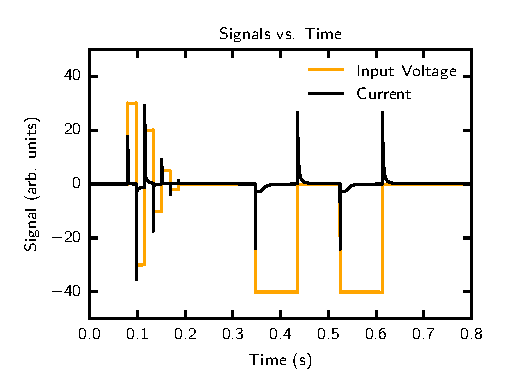
\includegraphics[scale=1]{figures/DLTS-waveform}
    
\includegraphics[scale=1]{figures/snippet-single}
    \caption[DLTS excitation waveform and single transient response]{DLTS excitation waveform and representative single-pulse transient response. The left panel shows the applied voltage pulses together with the corresponding current response. The right panel compares the charge and discharge transients after one pulse, showing a fast initial response followed by a slower relaxation towards the baseline.}
    \label{fig:dlts_waveform_single_transient}
\end{figure}

Figure~\ref{fig:dlts_waveform_single_transient} shows the pulse sequence and a representative single transient. The sharp current peaks at the voltage edges originate mainly from the rapid charging or discharging of the device capacitance. After this initial response, the current decays more gradually. The charge and discharge branches have opposite signs, which is expected because the electric field drives carriers into or out of trap states depending on the direction of the voltage step. The non-instantaneous return to the baseline indicates that the OFET response is not purely capacitive, but also contains slower trapping and detrapping processes.

For a qualitative interpretation, the transient current can be considered as a sum of relaxation components,
\begin{equation}
I(t)=I_\infty+\sum_i A_i\exp\left(-\frac{t}{\tau_i}\right),
\end{equation}
where $I_\infty$ is the long-time background current, $A_i$ is the amplitude of a relaxation component, and $\tau_i$ is the corresponding characteristic time constant. A single exponential would indicate one dominant trap time scale, whereas a broader or multi-exponential decay indicates a distribution of trap depths and local environments~\cite{Lang1974DLTS,Williams1970KWW,Elton2018StretchedExponential}. The measured traces show a rapid initial drop followed by a longer tail, which is consistent with a broad trap distribution typical of disordered organic semiconductor films.

\begin{figure}[htbp]
    \centering
    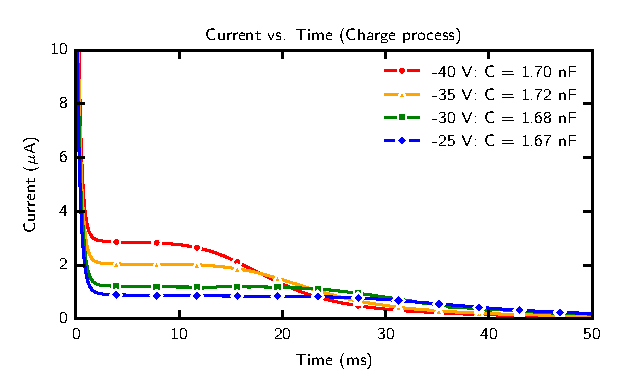
\includegraphics[scale=1.1]{figures/snippet-full}
    \caption[Full DLTS transient trace]{Full DLTS transient trace recorded during the charge process for different applied bias levels. The current relaxes after the voltage step and approaches a low background value. The effective capacitance is determined from $C_\text{eff}=Q/V_0$, with $Q$ obtained by integrating the transient current. The extracted values remain close to \SI{1.7}{\nano\farad}, indicating that the dominant fast contribution is capacitive, while the slower tail is associated with trap-related relaxation.}
    \label{fig:dlts_full_transient}
\end{figure}

The full transient trace in Figure~\ref{fig:dlts_full_transient} shows that the current relaxation depends on the applied bias. Larger voltage steps produce larger initial currents because more charge is displaced at the semiconductor--dielectric interface. Integrating each transient gives the displaced charge $Q$, and division by the corresponding voltage step gives the effective capacitance. At longer times, the traces converge towards a small residual current, indicating that the device approaches a stable state after the trap population has partially re-equilibrated. The extracted capacitance values are all close to \SI{1.7}{\nano\farad}, so the geometric and interfacial capacitance contribution is nearly constant over this voltage range. The remaining bias-dependent tail is therefore attributed mainly to the slow filling and emptying of localized trap states rather than to a change in the device capacitance itself.

Overall, the DLTS-type experiment confirms that the OFET contains slow relaxation processes that are not visible from the static transfer curve alone. These processes can influence threshold-voltage extraction and apparent mobility when measurements are performed with different sweep rates or after different bias histories~\cite{Bobbert2012OperationalStability,Hirwa2015TrapStates}. This observation supports the use of careful bias protocols and contact-independent analysis methods in the following characterization.

\subsection{Amplification Properties Analysis}

The OFET was also tested in a simple amplifier configuration to evaluate whether the measured field-effect modulation can be used in an electronic circuit. The aim of this measurement is not to optimize a practical amplifier, but to demonstrate that changes in gate voltage can be converted into measurable changes in output voltage. This provides an additional, circuit-level confirmation of transistor action.

\begin{figure}[htbp]
\centering
\resizebox{0.65\textwidth}{!}{\begin{circuitikz}[scale=0.5]
\ctikzset{resistor = european}
\ctikzset{tripoles/mos style/arrows}


\draw (-4,-4)--(-4,-6)--(-6,-6) to[R,l_=$R_S$] (-6,-10)--(-2,-10) to[C,l_=$C_S$] (-2,-6)--(-4,-6);
\draw (-4,-10)--++(0,-2) node[rground]{};

\draw (-4,4)to[short,-*](-4,7)to[R,l=$R_D$,-*](-4,11);
\draw (-4,7) to[C,l=$C_o$] (0,7);
\draw[->,blue](0,7)--++(2,0) node[right=1pt]{Output signal};
\draw[->,red] (-4,11)--++(0,2) node[right=1pt]{$V_\text{DD}$};
\draw (-4,0)to[short,-*](-10,0) to[C,l=$C_i$] (-14,0);
\draw[->,blue] (-14,0)--++(-1,0) node[left=1pt]{Input signal};
\draw (-4,11)--(-10,11) to[R,l=$R_1$](-10,0) to[R,l=$R_2$](-10,-11)to[short,-*](-4,-11) ;
\draw[black, fill = cyan!50, fill opacity = 0.3, line width = 1pt](-5,-5)--(5,-5)--(5,5)--(-5,5)--(-5,-5);

% Gate layer
\filldraw[line width = 1pt,fill = black!40, fill opacity = 0.5]
(-1.5,2.25)--(1.5,2.25) arc[start angle = 180, end angle = -90, radius = 0.75]
--(2.25,0.75)--(4,0.75) arc[start angle = 90, end angle = -90, radius = 0.75]--(2.25,-0.75)
--(2.25,-1.5) arc[start angle = 90, end angle = -180, radius = 0.75] --(-1.5,-2.25)
arc[start angle = 0, end angle = -270, radius = 0.75]--(-2.25,-0.75)
--(-4,-0.75) arc[start angle = -90, end angle = -270, radius = 0.75]--(-2.25,0.75)
--(-2.25,1.5) arc [start angle = -90, end angle = -360, radius = 0.75]
;
\draw[fill = black!40, fill opacity = 0.5, line width = 1pt](-4,-4) circle (0.75);
 \draw[fill = black!40, fill opacity = 0.5, line width = 1pt](-4,4) circle (0.75);
  \draw[fill = black!40, fill opacity = 0.5,line width = 1pt](4,4) circle (0.75);
 \draw[fill = black!40, fill opacity = 0.5,line width = 1pt](4,-4) circle (0.75);

% Insulator
\filldraw[draw=black, fill=blue!80, fill opacity=0.3, line width = 1pt]
(-4.5,-2.7)[sharp corners]--(-4.5,-0.9)[rounded corners=2ex]
--(-2.7,-0.9)--(-2.7,0.9)[sharp corners]--(-4.5,0.9)
--(-4.5,2.7)[rounded corners=2ex]--(-2.7,2.7)[sharp corners]--(-2.7,4.5)
--(2.7,4.5)[rounded corners=2ex]--(2.7,2.7)[sharp corners]--(4.5,2.7)
--(4.5,0.9)[rounded corners=2ex]--(2.7,0.9)--(2.7,-0.9)[sharp corners]--(4.5,-0.9)
--(4.5,-2.7)[rounded corners=2ex]--(2.7,-2.7)[sharp corners]--(2.7,-4.5)
--(-2.7,-4.5)[rounded corners=2ex]--(-2.7,-2.7)[sharp corners]--(-4.5,-2.7)
--cycle;


% Semiconductor layer
\path[fill=green, fill opacity=0.5, draw=green!50!black, line width=1pt]
    (0.7557,2.1193)
    arc[start angle=70.3746, end angle=109.6254, radius=2.25]
    arc[start angle=355.0011, end angle=634.9989, radius=1.5]
    arc[start angle=160.3746, end angle=199.6254, radius=2.25]
    arc[start angle=85.0011, end angle=364.9989, radius=1.5]
    arc[start angle=250.3746, end angle=289.6254, radius=2.25]
    arc[start angle=175.0011, end angle=454.9989, radius=1.5]
    arc[start angle=340.3746, end angle=379.6254, radius=2.25]
    arc[start angle=265.0011, end angle=544.9989, radius=1.5]
    -- cycle;


% Injection pads
\draw[red!90, draw opacity=0.7, line width=1cm, line cap=round, line width = 20pt](-2.25,-2.25) -- (-4,-4);
\draw[red!90, draw opacity=0.7, line width=1cm, line cap=round, line width = 20pt](2.25,-2.25) -- (4,-4);
\draw[red!90, draw opacity=0.7, line width=1cm, line cap=round, line width = 20pt](-2.25,2.25) -- (-4,4);
\draw[red!90, draw opacity=0.7, line width=1cm, line cap=round, line width = 20pt](2.25,2.25) -- (4,4);



% Contact pads
\draw[fill=orange, line width = 1pt](-4,-4) circle (0.75) node []{4};
 \draw[fill=orange, line width = 1pt](-4,4) circle (0.75) node []{3};
  \draw[fill=orange,line width = 1pt](4,4) circle (0.75) node []{2};
 \draw[fill=orange,line width = 1pt](4,-4) circle (0.75) node []{1};
 \draw[fill=orange,line width = 1pt](-4,0) circle (0.75) node []{G};
 \draw[fill=orange,line width = 1pt](4,0) circle (0.75) node []{G};



\end{circuitikz}}
\caption[OFET amplification measurement circuit]{Circuit used to analyse the amplification properties of the OFET. The input signal is capacitively coupled to the gate through $C_i=\SI{1}{\nano\farad}$, while the gate operating point is set by the bias divider with $R_2=\SI{100}{\kilo\ohm}$ and variable $R_1$. The drain is biased through $R_D$ at $V_\text{DD}=\SI{-30}{\volt}$, with $R_D$ varied from \SI{20}{\mega\ohm} to \SI{50}{\mega\ohm}. The output signal is measured at the drain contact through $C_o=\SI{1}{\nano\farad}$. The source branch contains $R_S$ and the bypass capacitor $C_S=\SI{1}{\nano\farad}$, which set the source bias and influence the small-signal response.}
\label{fig:ofet_amplification_circuit}
\end{figure}

Figure~\ref{fig:ofet_amplification_circuit} shows the common-source amplifier circuit used for this test. The gate bias defines the operating point of the OFET; it was adjusted with the variable resistor $R_1$ together with $R_2=\SI{100}{\kilo\ohm}$. The coupling and bypass capacitors were all \SI{1}{\nano\farad}. The drain resistor $R_D$, assembled from load-resistor combinations between \SI{20}{\mega\ohm} and \SI{50}{\mega\ohm}, converts a modulation of channel current into a voltage signal at the output. Because the device is a $p$-type transistor operated with a negative supply voltage, the sign convention differs from that of a standard $n$-channel amplifier, but the small-signal principle is the same: a change in gate voltage changes the channel current, and this current change produces a voltage drop across the load resistor~\cite{Neamen,Lundstrom2023Transistors}.



The static amplifier characteristics are shown in Figure~\ref{fig:ofet_transfer_amplification}. At small input voltages the channel is weakly accumulated, while at large input voltages it is already close to strong accumulation. The strongest gate control therefore occurs in the intermediate range, where the output voltage changes most rapidly. The gain is negative, as expected for a common-source stage, and increases in magnitude when $R_D$ is raised from \SI{20}{\mega\ohm} to \SI{50}{\mega\ohm}. This larger load resistance also increases the influence of parasitic capacitances, so the highest-gain setting is not necessarily the fastest or most linear operating point.


Figure~\ref{fig:ofet_amplifier_dynamic_response} shows the response to sinusoidal and square-wave inputs. The sinusoidal output is phase-inverted and larger than the input, confirming voltage amplification. The rounded waveform and the finite rise and fall times in the square-wave response show that the bandwidth is limited by the large load resistance, device and wiring capacitances, and trap-related relaxation~\cite{Bobbert2012OperationalStability,Hirwa2015TrapStates}. The output nevertheless follows the input reproducibly, so the OFET can operate as an active amplifying element under the chosen bias conditions.

Together with the DLTS results, this measurement shows that the devices combine useful field-effect modulation with significant dynamic effects. Contact effects, trap states, and time-dependent charging must therefore be considered when extracting quantitative parameters or designing circuits based on these OFETs.

\begin{figure}[htbp]
    \centering
    
\includegraphics[scale=1]{figures/oFET-transfer}
    
\includegraphics[scale=1]{figures/oFET-amp}
    \caption[OFET transfer curve and amplification characteristic]{OFET transfer curve and amplification characteristic at $V_\text{DD}=\SI{-30}{\volt}$ for different drain-load resistances $R_D$. The transfer plot identifies the input-voltage range where the output voltage changes most strongly, while the amplification plot shows the corresponding small-signal voltage gain. Larger $R_D$ values increase the maximum gain but also narrow the useful operating range.}
    \label{fig:ofet_transfer_amplification}
\end{figure}


\begin{figure}[htbp]
    \centering
    
\includegraphics[scale=1]{figures/amp-response-sin}
    
\includegraphics[scale=1]{figures/amp-response-square}
    \caption[Dynamic response of the OFET amplifier]{Dynamic response of the OFET amplifier at $V_\text{DD}=\SI{-30}{\volt}$, $R_D=\SI{50}{\mega\ohm}$, $V_\mathrm{G,Q} = \SI{-18}{\volt}$, and $f=\SI{10}{\kilo\hertz}$. The sinusoidal measurement demonstrates inverted voltage amplification, while the square-wave measurement shows the finite rise and fall times caused by the large circuit resistance, device capacitance, and trap-related relaxation.}
    \label{fig:ofet_amplifier_dynamic_response}
\end{figure}
